
%cmd: clear; latex color.tex
%cmd: clear; xdvi color.dvi

% colors : white, black, red, green, blue, cyan, magenta, yellow.
% dvips color names:


\documentclass[12pt]{article}
\usepackage[utf8]{inputenc}
\usepackage[english]{babel}
\usepackage{graphicx}
\usepackage[usenames,dvipsnames,svgnames,table]{xcolor}

%\usepackage{color}

\title{Assignment 1}
\author{Bhishan Poudel}
\date{August 2015}

\begin{document}
%  \pagecolor{declared-color}    % change color of whole page

\section{Qn.1}
\emph{some black text, \color{red} followed by a red fragment}, going black again.

\section{Qn.2}

{\color[rgb]{1,0,0} This text will appear red-colored}
\textcolor[rgb]{0,1,0}{This text will appear green-colored}

The 68 standard colors known to dvips

Invoke the package with the usenames and dvipsnames option. If you are using tikz or pstricks package you must declare the xcolor package before that, otherwise it will not work.




\indent This is indented text


\noindent This line is not indented





%%%%%%%%%%%%%%%%%%%%%%%%%%%%%%%%%%%%
\begin{figure}[ht!]
  \caption{dvips colors}
  \centering
    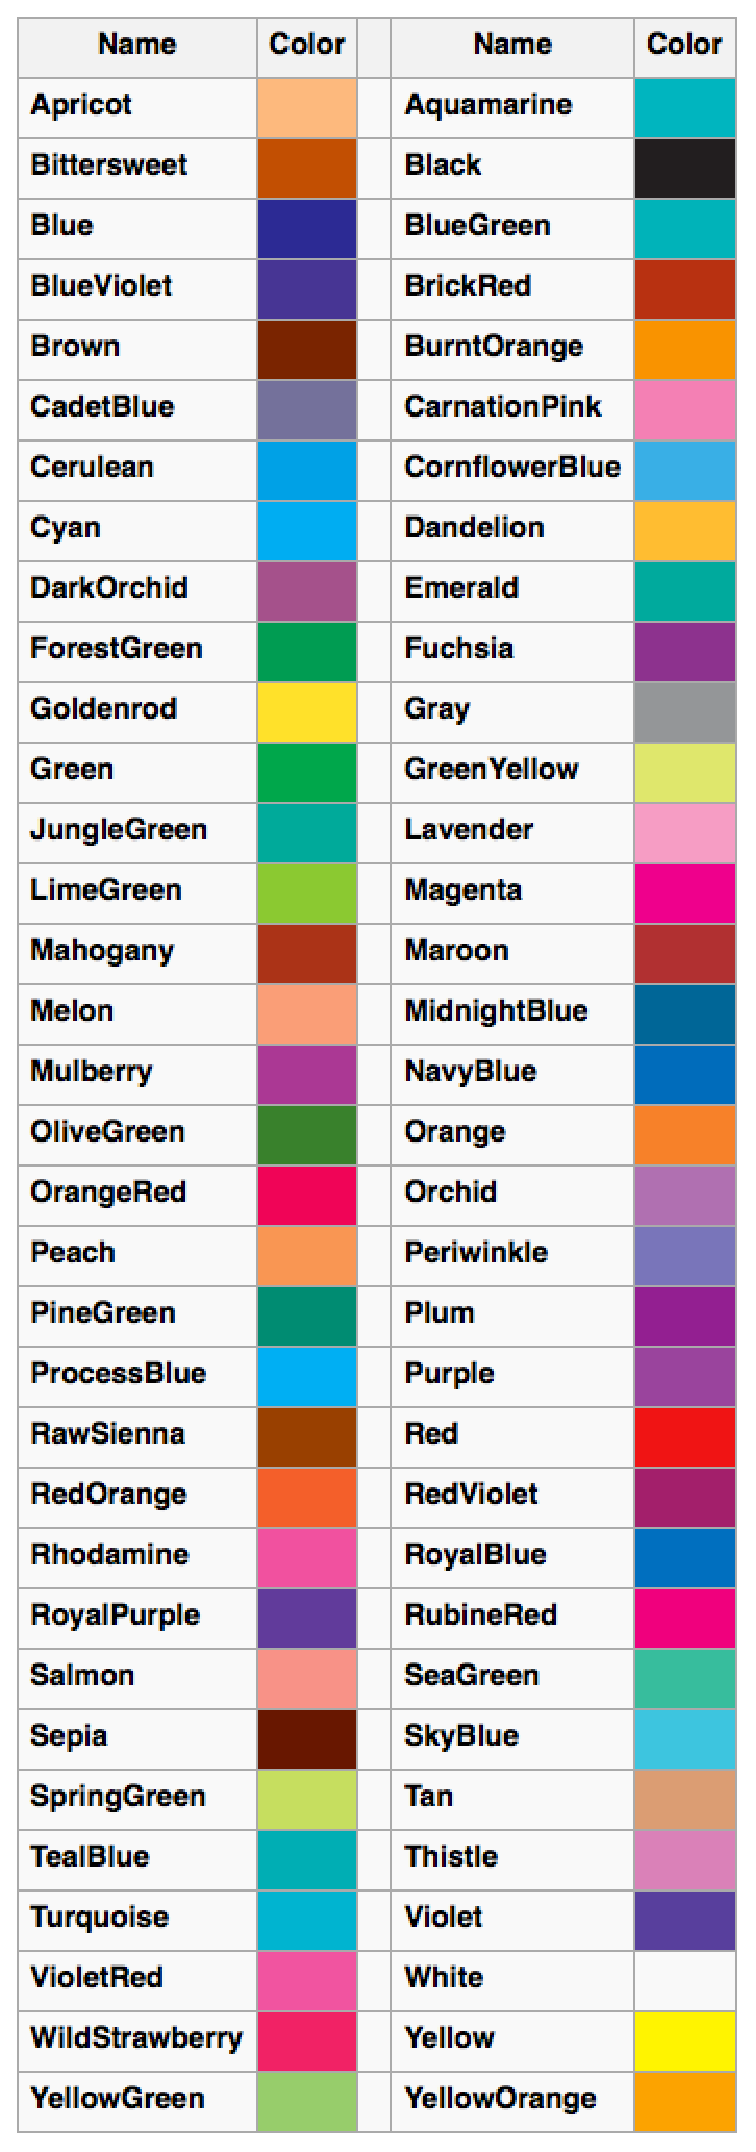
\includegraphics[width=0.5\textwidth]{dvipsColors.eps}
\end{figure}
%%%%%%%%%%%%%%%%%%%%%%%%%%%%%%%%%%%%%



\end {document}
